\documentclass[UTF8]{ctexart}

\usepackage[utf8]{inputenc}
\usepackage{lmodern}
\usepackage{amsmath}
\usepackage{cite}
\usepackage{xcolor}
\usepackage{listings}
\usepackage{graphicx}
\usepackage{float}
\usepackage{multirow}
\usepackage{booktabs}
\usepackage{natbib}

% 定义颜色
\definecolor{codegreen}{rgb}{0,0.6,0}
\definecolor{codegray}{rgb}{0.5,0.5,0.5}
\definecolor{codeorange}{rgb}{1,0.49,0}
\definecolor{backcolour}{rgb}{0.95,0.95,0.96}

\renewcommand\lstlistingname{源代码}
\renewcommand\lstlistlistingname{源代码}

\lstdefinestyle{mystyle}{
    backgroundcolor=\color{backcolour},   % Background color
    commentstyle=\color{codegray},        % Comment color
    keywordstyle=\color{codeorange},      % Keyword color
    numberstyle=\tiny\color{codegray},    % Line number style
    stringstyle=\color{codegreen},        % String style
    basicstyle=\ttfamily\footnotesize,    % Basic font style and size
    breakatwhitespace=false,              % Prevent line breaks at whitespace
    breaklines=true,                      % Enable automatic line breaking
    captionpos=b,                         % Caption position (bottom)
    keepspaces=true,                      % Preserve spaces
    numbers=left,                         % Line numbers on the left
    numbersep=5pt,                        % Spacing between numbers and code
    showspaces=false,                     % Do not show spaces as special characters
    showstringspaces=false,               % Do not show spaces in strings as special characters
    showtabs=false,                       % Do not show tabs as special characters
    tabsize=2,                            % Tab size (spaces per tab)
    xleftmargin=10pt                      % Left margin for the code block
}

\lstset{style=mystyle} % Apply the custom style

% 补充定义关键词函数
\providecommand{\keywords}[1]{
  \small
  \textbf{关键词:} #1
}

\title{图像去噪与分割算法寻根}
\author{大数据2201 万方}
\date{\today}

\begin{document}

\maketitle

\begin{abstract}
本文总结归纳了图像工程在图像去噪、图像分割等两大领域的多种经典方法,这些方法以其优雅的数学解释、精巧简洁的算法实现和出众的实现效果,启发了计算机视觉这一庞大学科的蓬勃发展。在深度学习算法广泛统治了整个计算机视觉、对算法可解释性需求愈发迫切的当下,这些传统的图像处理算法必然有其可以借鉴和深入发掘的价值。本文主要探究了全变差图像去噪算法(TV)与稀疏3D变换域协同滤波(BM3D),Graph\\Cut图像分割算法和互动式GrabCut图像分割算法。并具体地分析了两组传统算法间的优劣与特色,并分别给予了算法实现和效果比较,得到的结果是:TV在产业界应用相比于BM3D方法更为广泛的最大原因很有可能源于其在略弱的效果下实现了极高的性能,且拥有显著更简单的数学理论基础,而BM3D算法较大的计算量似乎并不能带来碾压性的性能提升,其价值与当今许多深度学习去噪方法一样,更多地在于理论性能的优越和学术发展的意义。而对于图像分割算法,基于大量数据预训练的深度学习模型已经能以更小的计算量实现较GrabCut更优越的分割结果,似乎分割算法相较于去噪算法可能会更不可避免地卷入深度学习的浪潮中。
\end{abstract}


\keywords{图像去噪\quad 图像分割\quad 全变差去噪\quad GrabCut}


\section{引言}
\subsection{图像去噪的研究进展}
在图像去噪领域,事实上一直有两种主要策略——区分性建模与优化性建模。\cite{tian_deep_2020}前者着眼于对图像中存在的真实噪音成分进行有效的建模,并通过“加性噪音”表示的形式采用逆过程消除噪声,其核心假设可以用一个简单的公式来表示:\par
\[y=x+n\]
而后者则将噪声视为一种图像中梯度规律性的高度不连续,其对图像去噪的理解为引导图像往更加平滑、更难检测出显著的微观不连续结构进行变换,并将这个过程理解为图像去噪的实现,这种策略往往不像区分性建模一样有对噪声的显式建模,而是让噪声在梯度下降或更为复杂的过程中被“自然地去除”。本文中将要重点复现和对比的两种方法分别属于二者,其中TV算法更强调对原图像主要梯度的保留及噪声的数学表示,而BM3D则更偏向于构造复杂的损失和模式匹配,隐式地去除图像的噪声。
\subsection{图像分割的研究进展}
自20世纪70年代以来,图像分割一直受到计算机视觉研究者的持续关注。经典的分割方法主要侧重于突出和提取单幅图像中所包含的信息,因此也通常需要专业知识和人为干预。且从根源上看,图像分割的核心是解决一下两个问题\cite{yu_techniques_2023}:
\begin{enumerate}
  \item 如何定义和表示“感兴趣区域(ROI)”
  \item 如何理解一幅图像中的“语义对象”
\end{enumerate}\par
在长期实践和探索中,基于对颜色和图像梯度信息的传统方法表现出往往难以从图像中获取高层次的语义信息的劣势。而较有效的协同分割方法涉及从一组图像中识别出共同的目标,这需要获取一定的先验知识(人工选取区域,而不是人工的细致标注)。由于这些方法对图像标注的依赖性较低,因此被归类为半监督或弱监督方法。随着大规模细粒度标注图像数据集的不断丰富,基于深度神经网络的图像分割方法逐渐成为一个热门研究课题。\par
由于深度学习模型在广泛的视觉应用中取得了巨大成功,许多研究致力于利用深度学习模型开发图像分割方法。\cite{minaee_image_2022}我对深度学习图像分割领域的多篇综述与数篇技术性论文进行了全面回顾,涵盖了语义分割和实例级分割领域中的一系列开创性工作,包括全卷积像素标记网络、编码器-解码器架构、多尺度与金字塔方法、循环网络、视觉注意力模型以及生成对抗模型。我领略了这些深度学习模型之间的相似性、优势与挑战,也对SegmentAnything等模型的在线Demo进行了尝试和评价。而在本文中,我将对传统的GrabCut及其互动式变体进行详细的复现与评价。

\section{TV:全变差图像去噪}
全变差图像去噪方法于1992年提出\cite{rudin_nonlinear_1992},是一种基于拉普拉斯方程的图像去噪方法。作为最早的一批具有良好效果和完善数学理论的传统图片去噪算法,其有着超越时代的优越性能,在当下去噪模型广泛采用深度学习方法的当下,依然被作为一个常用的参照项用于对比和性能分析。深入探讨全变差去噪算法,能够有效提高对图象去噪算法的认识。
\subsection{原理概况}
全变差(Total Variation, TV)去噪算法是一种常用的图像去噪技术,它通过正则化图像的梯度来减少噪声,同时保持图像的边缘细节。噪声通常会导致图像的像素值发生波动,尤其在图像的平坦区域,这种波动会产生不自然的细节。全变差方法的核心思想是通过抑制图像的梯度(即局部变化)来去除噪声,但又不抑制图像中的边缘部分。因为在自然图像中,边缘区域通常是图像的重要信息部分,不应当被平滑掉。全变差去噪通过在优化过程中引入一个正则化项来控制这一平衡,最大程度上保持图像的结构特征,如边缘,同时减少噪声的影响。

全变差去噪问题可以通过一个变分优化模型来描述,其优化目标是最小化图像的全变差和图像数据与原始图像的保真度之间的加权和。具体地,给定原始图像$u_0$,去噪后的图像为 $u$,全变差去噪的优化问题可以表示为:

\[
\min_u \left( \text{TV}(u) + \lambda \cdot \text{DataFidelity}(u) \right)
\]

其中,\( \text{TV}(u) \) 是图像的全变差,描述图像中像素值变化的总和。它的数学表达式为:

\[
\text{TV}(u) = \int_{\Omega} \|\nabla u(x)\|dx
\]

在离散图像中,全变差可以通过计算图像每个像素的梯度来进行近似。常见的计算方式是通过像素间的差分来计算梯度,得到如下离散化形式:

\[
\text{TV}(u) = \sum_{i,j} \sqrt{\left( \frac{\partial u}{\partial x} \right)^2 + \left( \frac{\partial u}{\partial y} \right)^2}
\]

这项全变差惩罚项的作用是平滑图像,减少不必要的噪声,但又不会影响图像的主要结构(如边缘)。另一方面,数据保真度项 \( \text{DataFidelity}(u) \) 衡量去噪后图像 \( u \) 与原始图像 \( u_0 \) 之间的差异。通常,这一项用平方差来度量,如下所示:

\[
\text{DataFidelity}(u) = \frac{1}{2} \| u - u_0 \|^2
\]

在优化过程中,数据保真度项确保了去噪后的图像尽量保留原始图像的特征,而全变差项则抑制图像中的噪声。最终,优化过程通过调整正则化参数 \( \lambda \),在保留图像细节和去除噪声之间找到一个平衡点。

全变差去噪通常通过数值优化方法求解,其中最常用的算法是梯度下降法和分裂算法。梯度下降法通过迭代更新图像 \( u \),使得目标函数逐渐减小,直到收敛。分裂算法则通过引入辅助变量,将原问题分解为一系列更容易求解的子问题。全变差去噪的关键优势在于它能够在去除噪声的同时保留图像的边缘结构,尤其适合处理图像中噪声较为显著的情况。
\subsection{效果浅析}
\subsubsection{numpy手工实现}
在这一部分,我将基于Matlab实现的一个TV算法在Python中使用numpy模块进行复现,并结合论文中的具体原理分析先过程中使用的具体策略和方法。首先,我们使用差分的方式遍历图像的每个像素点,计算每个像素点的四相梯度:
\begin{lstlisting}[language=Python, caption={梯度计算}, label={lst:code1}, mathescape=true, breaklines=true]
ux = (u[i + 1, j] - u[i, j]) / h
uy = (u[i, j + 1] - u[i, j - 1]) / (2 * h)
Gradu = np.sqrt(ux**2 + uy**2)
co1 = 1.0 / (Gradu + 1e-10)
  \end{lstlisting}

接着,据计算出的梯度,我们更新图像的像素值。图像的新值是由原图像值以及相邻像素的加权平均值组成。权重由梯度系数决定,而正则化参数决定了最终图片的平滑程度:
\begin{lstlisting}[language=Python, caption={引入正则}, label={lst:code2}, mathescape=true, breaklines=true]
u[i, j] = (
  u0[i, j]
  + (1 / (lambda_param * h * h)) * (
      co1 * u[i + 1, j]
      + co2 * u[i - 1, j]
      + co3 * u[i, j + 1]
      + co4 * u[i, j - 1]
  )
) * (
  1
  / (
      1
      + (1 / (lambda_param * h * h))
      * (co1 + co2 + co3 + co4)
  )
)
\end{lstlisting}

然后,为了保证图像边缘的像素值合理,我们在每次更新后对边界像素进行了特殊处理,采用最近邻的像素值来填充边界:
\begin{lstlisting}[language=Python, caption={领域填充}, label={lst:code3}, mathescape=true, breaklines=true]
u[1:M - 1, 0] = u[1:M - 1, 1]
u[1:M - 1, -1] = u[1:M - 1, -2]
\end{lstlisting}

最后,每次迭代结束后,我们计算当前图像的残差。残差是由图像的梯度和与原图像的差值构成的$L_1$损失,残差越小,表示图像越平滑,噪声越少:
\begin{lstlisting}[language=Python, caption={执行去噪}, label={lst:code4}, mathescape=true, breaklines=true]
en = 0.0
for i in range(1, M - 1):
    for j in range(1, N - 1):
        ux = (u[i + 1, j] - u[i, j]) / h
        uy = (u[i, j + 1] - u[i, j]) / h
        fid = (u0[i, j] - u[i, j]) ** 2
        en += np.sqrt(ux**2 + uy**2) + lambda_param * fid
loss.append(en)
\end{lstlisting}

通过以上步骤,我们成功地将Matlab中的全变差去噪算法(hpROF)用Python实现,并进行了详细的迭代过程分析,得到了如图\ref{fig:tvfromscratch}所示的最终的去噪结果。通过逐步更新图像像素值并计算每次迭代的能量,我们有效地去除了图像中的噪声,同时保持了图像的边缘信息。这个过程展示了在图像工程中的数学建模与编程实现的紧密结合。
% 手工实现TV去噪算法效果图
\begin{figure}[H]
  \centering
  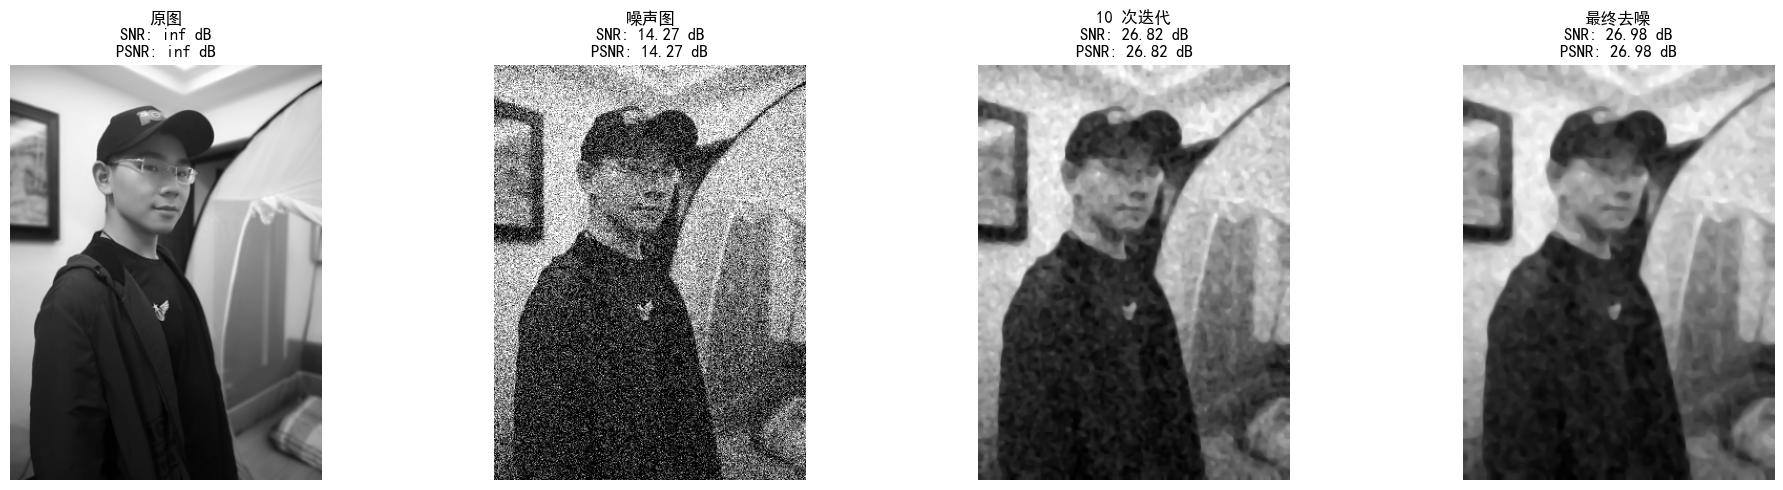
\includegraphics[width=\textwidth]{./images/tvfromscratch.png} 
  \caption{手工实现的TV去噪算法效果呈现}
  \label{fig:tvfromscratch}
\end{figure}

\subsubsection{拆解Scikit-image实现}
在这一部分,我将结合skimage对TV去噪算法的实现代码,对成熟的公开方法的实现思路进行拆解,并结合论文中的原理,对工程化实现过程中对初始算法进行的加速和优化进行解析。就实现而言,skimage中的实现在严格遵循了论文中的梯度投影法实现的同时,也引入了如下特性以增加其算法实现的稳健性:
\begin{enumerate}
  \item 支持多维图像
  \item 严格使用Chambolle算法加速计算
  \item 优化过程中的参数控制
  \item 给出了明确的收敛准则
\end{enumerate}
就具体而言,它实现了对任意维度的图像的支持,包括二维(灰度图像)和三维及更高维度的图像,能够处理多通道图像(如RGB图像),算法可以根据需要选择图像的通道进行处理。同时,使用了正则化参数$\lambda$的倒数。这个权重控制去噪的强度,权重越大,去噪效果越明显,但可能牺牲图像的细节保真度。通过一系列参数和方法的优化,算法能在去噪和保真度之间找到一个平衡点,实现如图\ref{fig:tvwithskimage}所示的最后一幅图的更优的去噪结果。
% 模块实现TV去噪算法效果图
\begin{figure}[H]
  \centering
  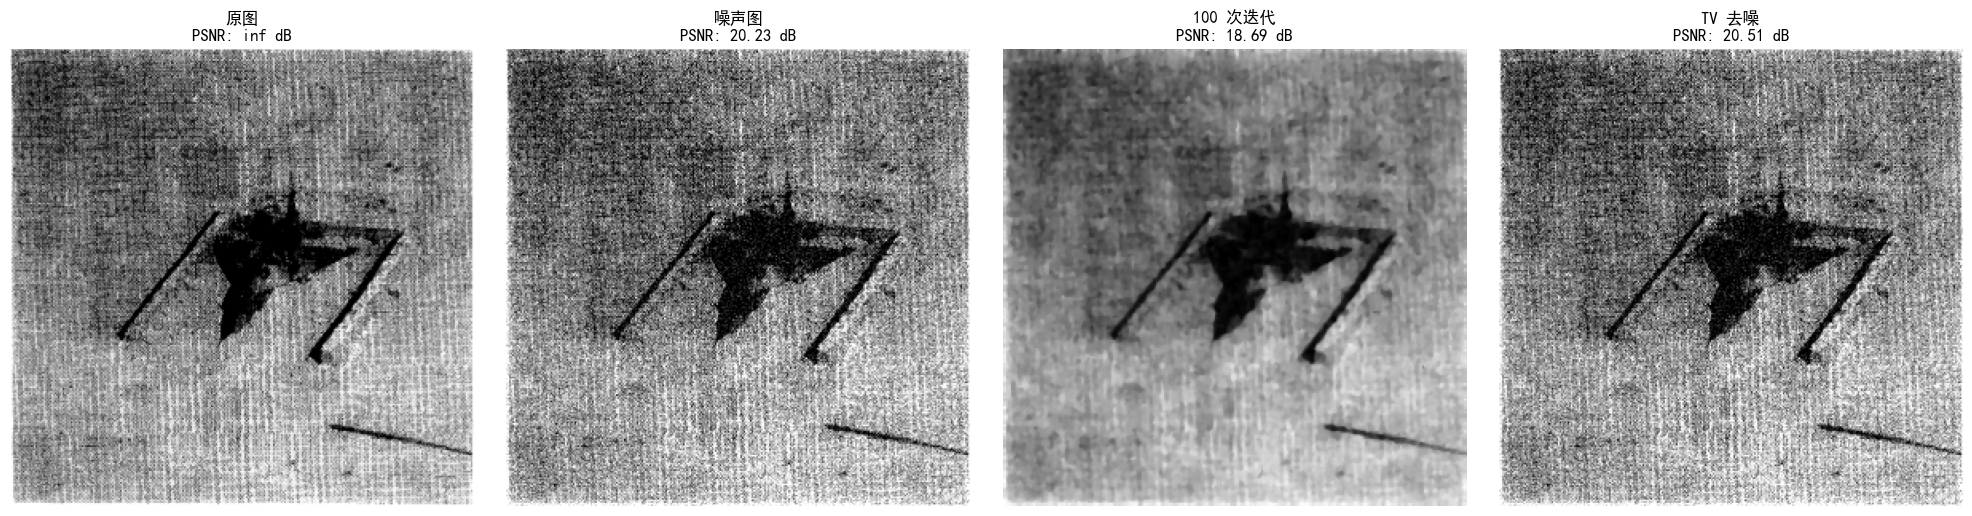
\includegraphics[width=\textwidth]{./images/tvwithskimage.png} 
  \caption{skimage模块实现的TV去噪算法效果呈现}
  \label{fig:tvwithskimage}
\end{figure}

\subsection{思考与总结}
在复现这两种全变差(TV)去噪算法的过程中,我深刻体会到了理论与实践之间的差异。skimage模块提供的TV算法通过Chambolle算法进行优化,支持多维数据的去噪,它在高维数据上的通用性和计算复杂度,真正实现了高效的实际应用。相比之下,我的复现代码(hpROF)实现相对简单,专注于二维图像的去噪,采用粗糙的逐像素更新的梯度下降方法,通过四个方向的梯度计算来调整像素值。尽管这种方法在性能上较为高效,但其缺乏明确的停⽌条件和计算精度的控制,也让我意识到简单算法在处理边界和复杂图像细节时可能存在一定的局限,而且在客观性能上也与完整实现有明显差异。不过总体而言,复现过程中让我更加理解了各类算法在不同应用场景下的适用性与实现细节,同时也让我更加重视算法的优化和参数调优在实际应用中的重要性。表\ref{tab:tvCompare}汇总了我对两个算法的全部对比与思考:
\begin{table}[htbp]
  \centering
  \caption{基于全变差(TV)去噪算法的对比}
  \label{tab:tvCompare}
  \begin{tabular}{ccc}
  \toprule[1.5pt]
  \textbf{特点} & \textbf{模块实现} & \textbf{手工实现} \\
  \midrule
  支持维度 & 任意维度图像 & 二维图像 \\
  求解方法 & Chambolle变分法 & 梯度下降法 \\
  停止条件 & 能量变化阈值 & 最大迭代次数 \\
  正则化参数 & 正则项$\frac{1}{\lambda}$ & 正则项$\lambda$ \\
  梯度计算 & 轴向梯度差异 & 四方向梯度差异 \\
  边界处理 & 推测内插扩展 & 明确邻域值处理 \\
  能量计算 & 能量变化判断 & 残差显示追踪 \\
  \bottomrule[1.5pt]
  \end{tabular}
\end{table}


\section{BM3D:稀疏3D变换域协同滤波}

\subsection{原理概况}
BM3D(Block-Matching and 3D Filtering)算法是一种2007年提出的广泛应用于图像去噪的非局部方法\cite{dabov_image_nodate},利用了图像中的自相似性。在该算法中,首先通过将图像划分为小块(patches)来捕捉局部信息。对于每个图像块,BM3D会寻找与其相似的邻域块,然后在这些块上执行3D滤波。具体来说,BM3D包含两个主要步骤:块匹配和3D变换滤波。\par
在块匹配步骤中,算法通过计算图像中所有可能位置的块之间的相似度,选择相似度最高的一组块。这些相似的块通过某种距离度量(如欧几里得距离)来进行匹配。对于图像中某个块,假设其为$x_i$,那么与其相似的块集合可以表示为:
\[
\{ x_j \mid \| x_i - x_j \|_2 \leq \tau \}
\]

其中,τ是一个阈值,用来确定相似块的匹配范围。匹配到的一组块会被堆叠成一个3D数据数组,形成一个3D卷积框架,在此基础上执行滤波。\par
接下来,BM3D对匹配到的块进行3D变换(如离散余弦变换,DCT),然后在变换域内应用硬阈值处理。变换后的数据可以通过以下公式表示:

\[
\hat{x}_k = \mathcal{T}^{-1}(\mathcal{T}(x_k) \cdot H)
\]

其中,$\mathcal{T}$代表3D变换(如DCT),$\hat{x}_k$是变换后的去噪数据,$H$是阈值函数,表示对变换系数的硬阈值处理。通过阈值去除噪声部分,保留图像的主要结构。\par
最后,BM3D通过将去噪后的块重新合成回原始图像中。为了避免由于块重叠带来的伪影,BM3D通常使用加权平均来重构最终的图像。假设重建后的图像块为y,合成过程可以表示为:

\[
y = \frac{\sum_i w_i \cdot \hat{x}_i}{\sum_i w_i}
\]

其中,$w_i$是加权系数,通常取决于每个块的相似度和信噪比。通过这个加权平均过程,BM3D能够有效地抑制噪声并保留图像细节。

\subsection{效果浅析}
\subsubsection{numpy手工实现}
为了更好、更完整地的实现BM3D并达到尽可能最优的效果,我们将计算过程划分为了“基础去噪”和“滤波平滑去噪”两步,我将分别介绍两个步骤的实现。\\
\textbf{基础滤波部分:}\\
首先,我对图像进行了小块分割在图像中找到与参考块相似的其他块,并计算它们之间的相似度:
\begin{lstlisting}[language=Python, caption={图像分块}, label={lst:code5}, mathescape=true, breaklines=true]
def Step1_Grouping(noisyImg, RefPoint, BlockDCT_all, BlockSize, ThreDist, MaxMatch, WindowSize):
    WindowLoc = SearchWindow(noisyImg, RefPoint, BlockSize, WindowSize)
    BlockPos = np.zeros((Block_Num_Searched, 2), dtype = int)
    BlockGroup = np.zeros((Block_Num_Searched, BlockSize, BlockSize), dtype = float)
    Dist = np.zeros(Block_Num_Searched, dtype = float)
    RefDCT = BlockDCT_all[RefPoint[0], RefPoint[1], :, :]
    match_cnt = 0
    for i in range(WindowSize-BlockSize+1):
        for j in range(WindowSize-BlockSize+1):
            dist = Step1_ComputeDist(RefDCT, SearchedDCT)
            if dist < ThreDist:
                BlockPos[match_cnt, :] = [WindowLoc[0, 0] + i, WindowLoc[0, 1] + j]
                BlockGroup[match_cnt, :, :] = SearchedDCT
                Dist[match_cnt] = dist
                match_cnt += 1
    if match_cnt <= MaxMatch:
        BlockPos = BlockPos[:match_cnt, :]
        BlockGroup = BlockGroup[:match_cnt, :, :]
    else:
        idx = np.argpartition(Dist[:match_cnt], MaxMatch)
        BlockPos = BlockPos[idx[:MaxMatch], :]
        BlockGroup = BlockGroup[idx[:MaxMatch], :]
    return BlockPos, BlockGroup
\end{lstlisting}

接着,对找到的相似块进行3D变换和硬阈值处理,去除一些低于阈值的系数,达到噪声去除的效果:
\begin{lstlisting}[language=Python, caption={阈值处理}, label={lst:code6}, mathescape=true, breaklines=true]
def Step1_3DFiltering(BlockGroup):
    ThreValue = lamb3d * sigma
    for i in range(BlockGroup.shape[1]):
        for j in range(BlockGroup.shape[2]):
            ThirdVector = dct(BlockGroup[:, i, j], norm = 'ortho')
            ThirdVector[abs(ThirdVector[:]) < ThreValue] = 0.
            BlockGroup[:, i, j] = list(idct(ThirdVector, norm = 'ortho'))
    return BlockGroup
\end{lstlisting}

然后,对所有估算的块进行加权平均以得到最终的基本估计图像,呈现在图\ref{fig:bm3dfromscratch}的第三幅。\\
\textbf{滤波平滑去噪:}\\
首先,是和第一步一样的分块计算相似度。\\
然后是额外的\textbf{Wiener滤波},以进一步去除噪声:
\begin{lstlisting}[language=Python, caption={滤波平滑}, label={lst:code7}, mathescape=true, breaklines=true]
def Step2_3DFiltering(BlockGroup_basic, BlockGroup_noisy):
    for i in range(BlockGroup_noisy.shape[1]):
        for j in range(BlockGroup_noisy.shape[2]):
            Vec_basic = dct(BlockGroup_basic[:, i, j], norm = 'ortho')
            Vec_noisy = dct(BlockGroup_noisy[:, i, j], norm = 'ortho')
            Vec_value = Vec_basic**2 * coef
            Vec_value /= (Vec_value + sigma**2)
            Vec_noisy *= Vec_value
            BlockGroup_noisy[:, i, j] = list(idct(Vec_noisy, norm = 'ortho'))
    return BlockGroup_noisy
\end{lstlisting}
最后再次和第三步一样对分块加权平均得到最终去噪估计,并不断循环滤波平滑去噪直到处理前后差异小于阈值,得到如图\ref{fig:bm3dfromscratch}的最后一幅图的最终去噪结果,效果优异。\par

% 手工实现BM3D去噪算法效果图
\begin{figure}[H]
  \centering
  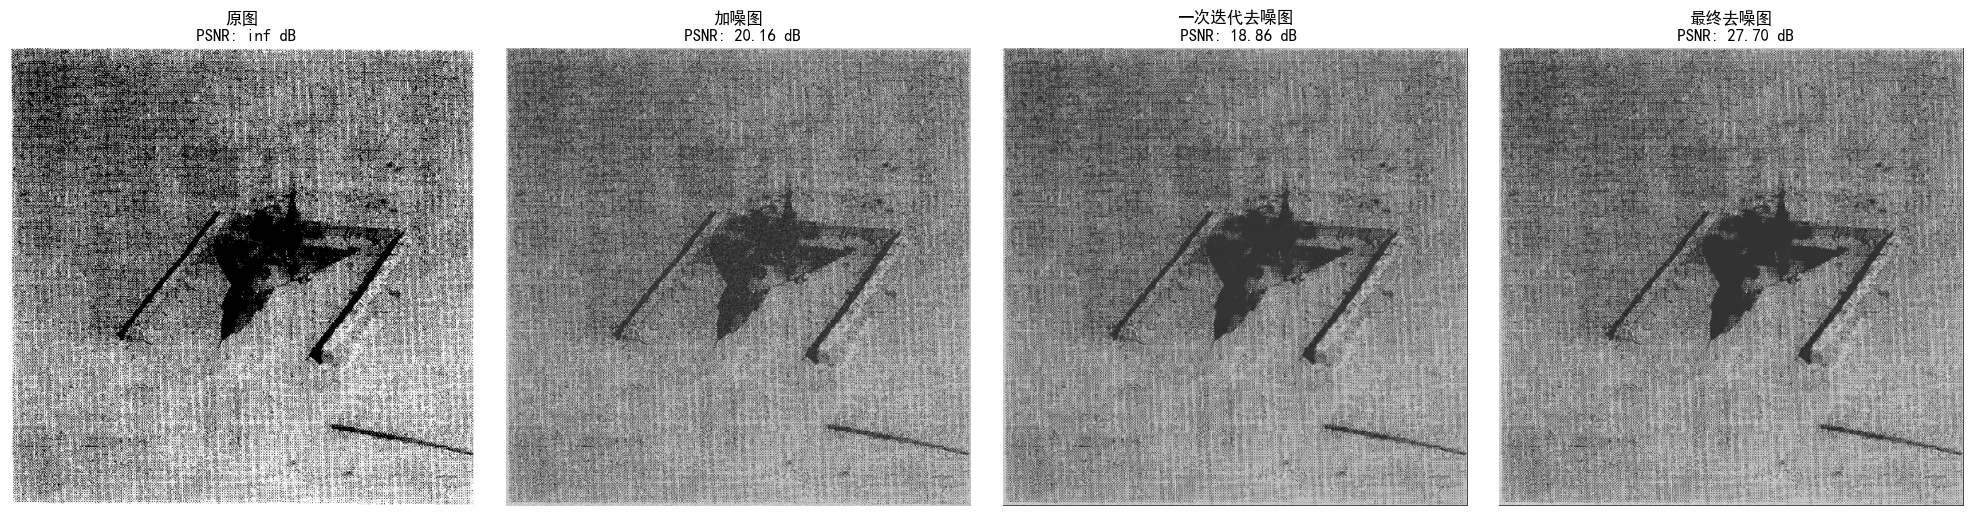
\includegraphics[width=\textwidth]{./images/bm3dfromscratch.png} 
  \caption{手工实现的BM3D去噪算法效果呈现}
  \label{fig:bm3dfromscratch}
\end{figure}
不过在调参和测试算法的过程中,我也注意到了一些有趣的现象,BM3D方法对于黑色的椒噪声和黑色成分较多的高斯噪声时似乎相对会敏感很多,在测试过程中经常会出现如图\ref{fig:bm3dwrong}所示的情况:
\begin{figure}[H]
  \centering
  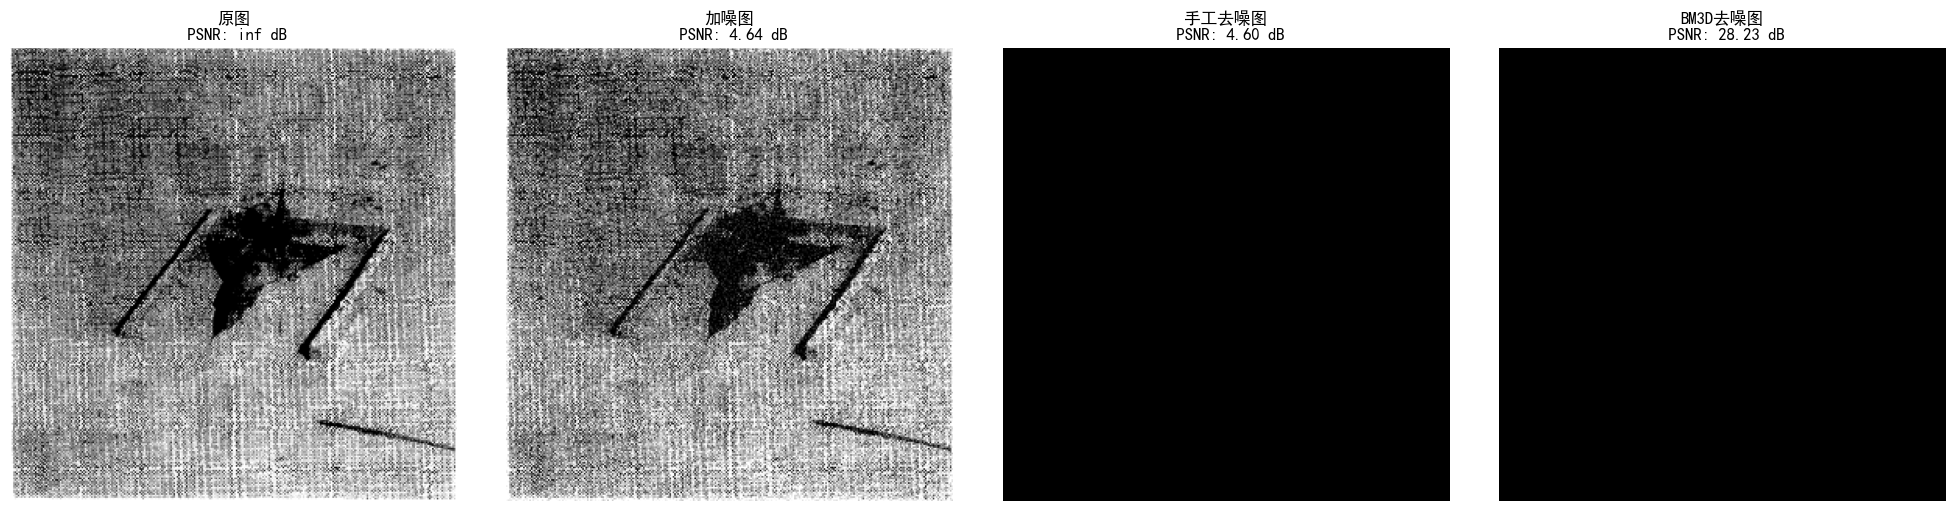
\includegraphics[width=\textwidth]{./images/bm3dwrong.png} 
  \caption{对椒噪声和高斯噪声的去噪效果}
  \label{fig:bm3dwrong}
\end{figure}
我猜测,这可能是噪声中含有大量与图像边缘元素相同的模式引起的。



\subsection{体会与思考}
有趣的是,对于BM3D,我并未找到可以模块化实现的包,即使有,也可能因为版本古早而无法使用pip安装,不过鉴于手动实现的效果良好,就不强求使用模块来对比实现了.\par
而从测试结果来看,BM3D的效果比模块实现的TV略好,但是对于噪声含有大量与图像边缘元素相同的模式,模型的敏感性交强,同时在计算过程方面BM3D的算法明显较TV更加复杂,也在计算速度上有明显劣势。时间对比如表\ref{tab:timecompare}所示。
\begin{table}[htbp]
  \centering
  \caption{TV算法与BM3D算法去噪同一个图像的时间对比}
  \label{tab:timecompare}
  \begin{tabular}{cccccc}
    \toprule[1.5pt]
    \multirow{2}{*}{方法} & \multirow{2}{*}{输入} & \multicolumn{2}{c}{计算时长(秒)} & \multirow{2}{*}{最高PSNR} \\
    \cline{3-4}
                           &                       & \text{一次迭代} & \text{最终结果} & \\
    \midrule
    \text{TV算法}           & \text{noised\_dntest.png} & \textbf{0.538*}  & \textbf{11.27*}  & \text{20.51} \\
    \text{BM3D算法}         & \text{noised\_dntest.png} & \text{43.40}  & \text{61.54}  & \textbf{28.86*} \\
    \bottomrule[1.5pt]
  \end{tabular}
\end{table}





\section{GraphCut \& GrabCut:静态与交互式的对比和拓展}
GraphCut是一种于2001年提出的常用于图像分割的算法\cite{boykov_interactive_2001},基于图论的最小割问题。图像分割的目标是将图像划分为不同的区域,GraphCut算法通过构造一个图,并通过最小化割的代价来实现分割。图的节点代表图像中的像素,而边则表示像素之间的关系。每一对相邻像素之间的边连接了它们的相似性(通常是颜色或亮度的相似性)。GraphCut算法的核心思想是通过最小化一个能量函数来找到最佳的像素划分。\par
该能量函数由两部分组成:数据项和光滑项。数据项衡量像素分配到某个类的代价,而光滑项则惩罚相邻像素分配到不同类的情况。数据项通常用像素与前景或背景的相似性来表示,而光滑项则考虑到图像中像素之间的相似性。能量函数的形式可以表示为:
\[
E(f) = \sum_i D_i(f_i) + \sum_{i,j} V_{ij}(f_i, f_j)
\]
其中,$f_i$是像素$i$的标签,$D_i(f_i)$是数据项,$V_{ij}(f_i, f_j)$是光滑项。数据项$D_i(f_i)$通常是像素与前景或背景的相似度,光滑项$V_{ij}(f_i, f_j)$则是相邻像素之间的相似性。\par
GraphCut问题的目标是通过最小化能量函数来找到最优的分割。该问题可以通过最大流最小割定理进行求解。最大流最小割定理表明,图的最小割等于图中最大流的值。GraphCut算法通过构造一个流网络,其中源点与前景之间连接,汇点与背景之间连接,然后计算最小割(即最大流)。这个最小割的结果对应于图像的分割结果。\par
通过最小化能量函数,GraphCut算法能够有效地将图像分割为前景和背景。其核心公式涉及最小割、最大流以及数据项和光滑项的优化。
\subsection{原理概况}
于2004年发表GrabCut算法是一种基于GraphCut的交互式图像分割方法\cite{rother_grabcut_2004},主要通过能量最小化实现前景和背景的分割。其核心原理是将图像表示为一个图(graph),以像素作为节点,并定义边权重来表示像素之间的关系。算法通过高斯混合模型建模颜色分布,并采用迭代优化的方式逐步精化分割结果。\par
在GrabCut中,能量函数的目标是最小化以下表达式:

\[
E(\alpha, \theta, z) = U(\alpha, \theta, z) + V(\alpha, z)
\]

其中,$\alpha$表示像素的前景或背景标签,$\theta$是图像的前景和背景颜色分布模型参数,$z$\\是像素的颜色值。能量函数由数据项$U$和光滑项$V$组成:\\
1. 数据项描述每个像素的颜色与前景或背景分布的相似性:
\[
U(\alpha, \theta, z) = \sum_{n} -\log P(z_n | \alpha_n, \theta)
\]
这里,\(P(z_n | \alpha_n, \theta)\)是由高斯混合模型定义的概率密度函数。\\
2. 光滑项描述像素标签的空间一致性,鼓励相邻像素具有相同标签:
\[
V(\alpha, z) = \gamma \sum_{(m,n)\in C} [\alpha_m \neq \alpha_n] \exp(-\beta \|z_m - z_n\|^2)
\]
其中,\(C\)是像素邻域集合,\(\beta\)用于调节颜色差异对光滑性的影响。\\
GrabCut通过迭代步骤优化上述能量函数,包括:\\
1. 基于当前分割更新高斯混合模型的参数;\\
2. 使用最小割算法更新像素标签,解决全局优化问题:
\[
\hat{\alpha} = \arg\min_{\alpha} E(\alpha, \theta, z)
\]

这种迭代过程保证能量函数逐步减少,直到收敛到局部最优解。通过用户交互(如矩形框选和划线标注)初始化分割区域,GrabCut能有效地分割复杂场景中的前景对象。
\subsection{效果浅析}
出于时间压力和一小部分惰性,我主要实现了对GrabCut的调用测试(并且原以为框选分割是对GraphCut的实现),并尽力达到了良好的分割效果。测试的图片是我的个人照,并转为灰度单通道进行分割,对于GraphCut,我采用了静态非严格蒙版进行测试,得到了如图\ref{fig:GraphCut}的分割效果。
\begin{figure}[htbp]
\centering
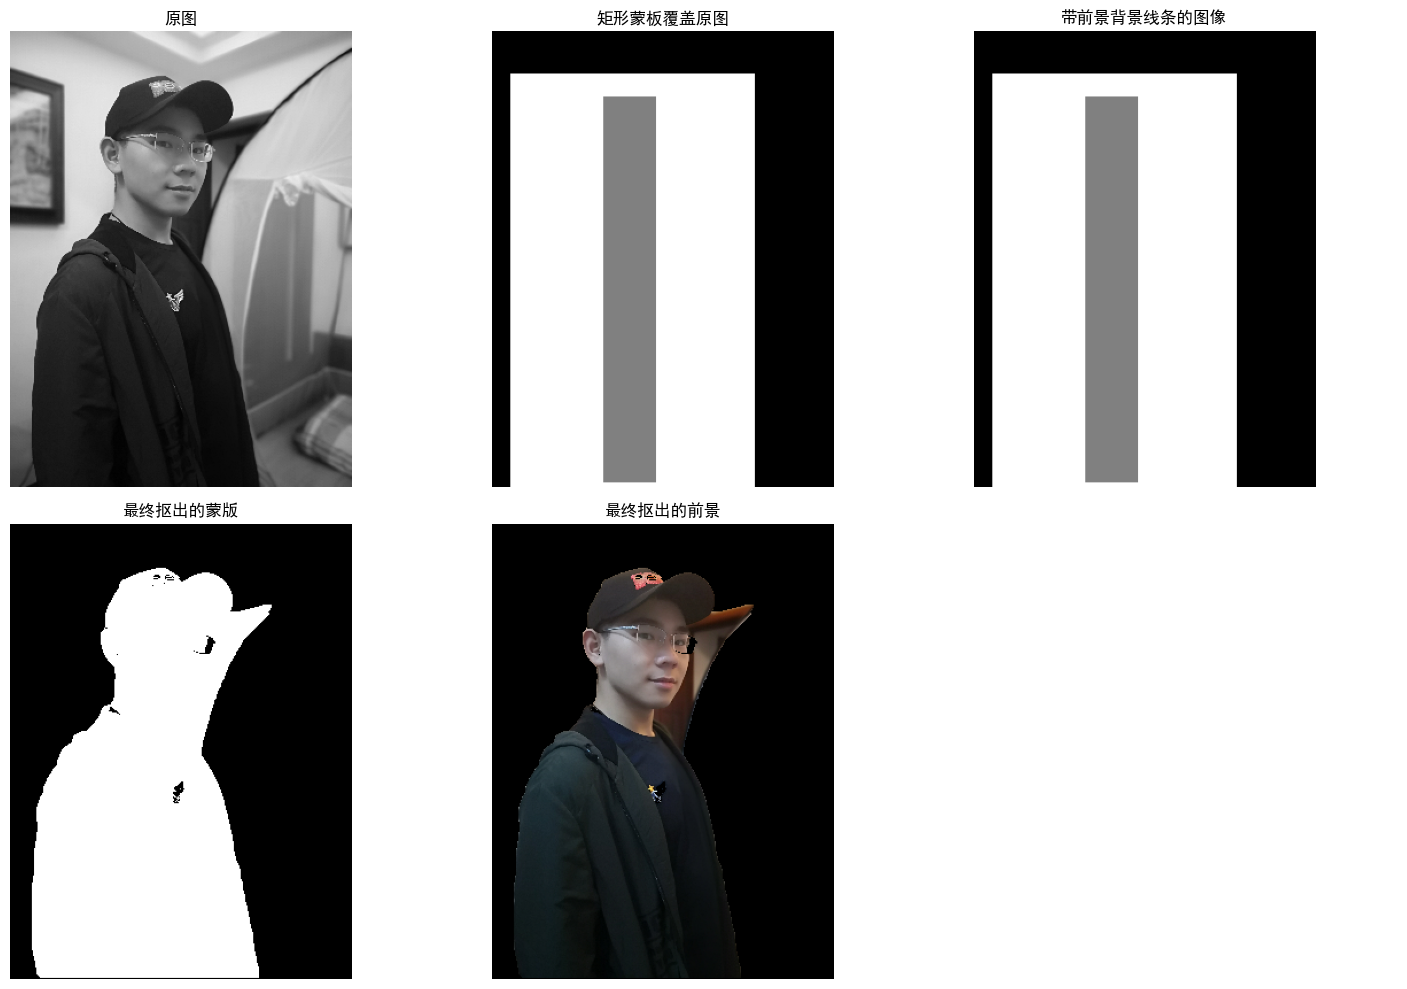
\includegraphics[width=0.8\textwidth]{./images/GraphCut.png}
\caption{GraphCut分割蒙版矩阵效果}
\label{fig:GraphCut}
\end{figure}

而对于GrabCut交互式图像分割算法,我们在粗糙前景蒙版标注作为基础分割的基础上,加入了画笔绘制严格前后景景的交互式标注,最终得到如图\ref{fig:GrabCut}更精确的分割结果。
\begin{figure}[H]
  \centering
  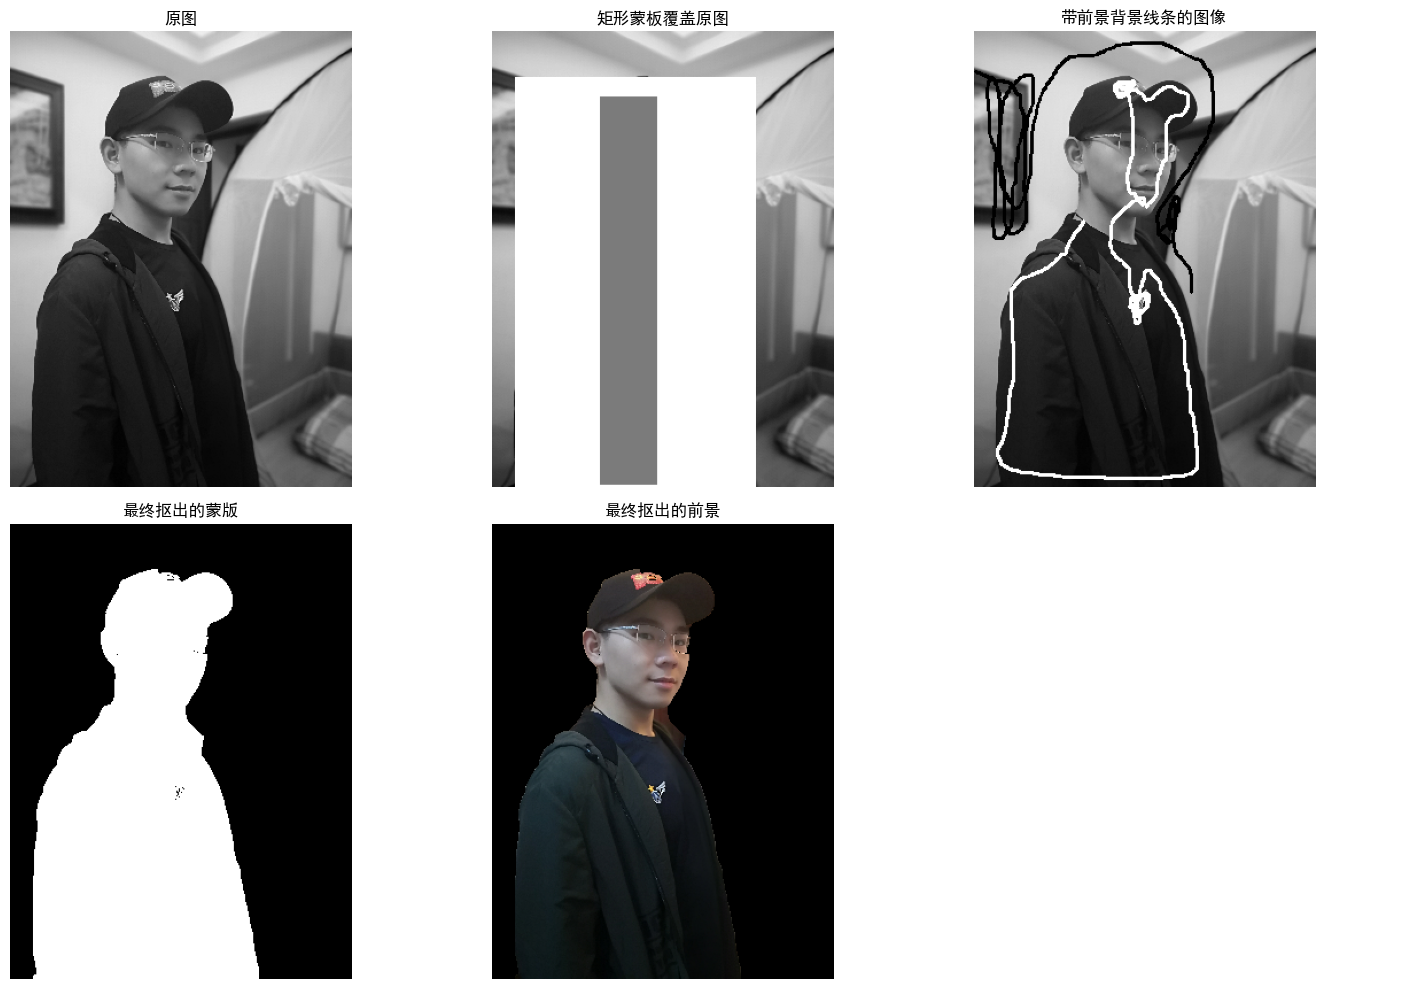
\includegraphics[width=0.8\textwidth]{./images/GrabCut.png}
  \caption{GrabCut分割蒙版矩阵效果}
  \label{fig:GrabCut}
  \end{figure}
其实我本来还想拆解一下OpenCV的实现源码,但在拆解过程中只在Opencv模块的\verb|__init__.pyi|文件中找到了\verb|cv2.rabCut|的doc,说明功能已经进行了编译封装,不便于拆解,也无意去开源项目里苦苦搜寻了,就介绍一下它的参数和调优过程吧。
\subsection{调优过程分析}
先介绍一下\verb|cv2.GrabCut|方法的所有参数吧:\par
\begin{table}[htbp]
\centering
\begin{tabular}{ccc}
\toprule[1.5pt]
\textbf{超参数} & \textbf{数据类型} & \textbf{描述} \\
\midrule
image & ndarray & 输入图像,8位或32位浮点图像 \\
mask & ndarray & 输入和输出蒙版图像,标记前景和背景 \\
rect & tuple & 用于初始化前景和背景的矩形框 \\
bgdModel & ndarray & 背景,5维高斯混合模型表示,1x65数组 \\
fgdModel & ndarray & 前景,5维高斯混合模型表示,1x65数组 \\
iterCount & int & 指定迭代次数,调整精度和速度 \\
mode & int & 模式,决定初始化方式和计算模式 \\
\bottomrule[1.5pt]
\end{tabular}
\caption{cv2.GrabCut 函数参数介绍}
\end{table}
本来最想测试的是负责前后景表示的\verb|fgdModel|与\verb|bgdModel|参数,从原理上讲,它是可能会提高每个GMM的维度可以增强模型的ROI表示能力,但鉴于整个模型已经被封装了,便无法做出改变,于是只能在10次内的迭代次数上对\verb|cv2.GC_INIT_WITH_RECT|\\和\verb|cv2.GC_INIT_WITH_MASK|进行测试和调参了,且\verb|mask|等其他参数我最初一直认为作为返回值回传即可,但在尝试手动实现的过程中注意到,由于Python的作用域范围限制,由用户创建并管理的可变数组在使用和修改过程中香蕉与返回值有更大的灵活性,因此也理解了这么设计的原因,不过,这也有可能是Java时代遗留的习惯所致。最终得到的参数组合如表\ref{tab:params}所示.

\begin{table}[htbp]
\centering
\begin{tabular}{cccc}
\toprule[1.5pt]
\textbf{mask} & \textbf{rect} & \textbf{iterCount} & \textbf{mode}\\
\midrule
\verb|GC_INIT_WITH_RECT结果| & \verb|框选| & \verb|7| & \verb|GC_INIT_WITH_MASK|\\
\bottomrule[1.5pt]
\label{tab:params}
\end{tabular}
\end{table}

\subsection{体会与思考}
在实现GrabCut算法的过程中,我深刻体会到了交互式图像分割的灵活性和高效性。GraphCut的静态分割虽然理论上能够提供精确的前景背景分割,但在实际应用中,图像内容的复杂性往往使得全自动的分割效果受到限制。尤其是当前景与背景之间的边界模糊或色彩相似时,静态方法难以做到理想的精度。\par
与之相比,GrabCut通过引入用户交互标注,大大提高了分割的准确度。通过框选和划线的方式,用户可以在初步分割的基础上进一步调整前景和背景区域,这样的交互式过程让算法能够在复杂场景中自适应地优化分割结果。这种方法不仅能减少算法对输入图像的依赖,还能提供一个直观且灵活的分割方案。\par
通过调参的过程,我逐步理解了如何通过合理设置迭代次数(iterCount)和初始化模式(mode)来达到更好的平衡。虽然初次使用时我对参数的作用理解并不透彻,但随着实验的深入,我发现通过调整这些超参数,能够在图像分割的速度和精度之间找到一个最佳的折中。\par
特别是mask和rect参数的作用,使得用户能够在粗略标注的基础上进一步优化模型。虽然最初我并未完全理解为什么掩膜需要在函数内外都进行传递,但通过对Python\\和Java中参数传递机制的对比,逐渐掌握了如何合理管理和修改可变对象。这一点对于图像处理中的复杂数据结构尤其重要。\par
总结来说,GrabCut作为一种交互式图像分割算法,给了用户更多的控制权,使得它在处理复杂图像时更加灵活。通过反复调整和测试不同的参数,我对算法的内在机制和调优过程有了更深入的理解,也更加意识到在实际项目中,灵活性和可交互性往往是算法成功的关键因素。

\section{总结}
本文通过对图像去噪与分割领域的两类经典算法——全变差去噪与稀疏3D变换域协同滤波去噪算法,以及基于GraphCut和GrabCut的图像分割算法的分析与实现,深入探讨了这些传统图像处理技术在实际应用中的表现与优势。\par
在去噪领域,TV算法凭借其简洁的数学理论和高效的计算性能,在工业界得到广泛应用。尽管其去噪效果在某些情况下略逊色于BM3D,但TV算法的优势在于其计算效率,尤其适合大规模数据处理。相比之下,BM3D算法虽然在理论性能上具有优势,但其计算复杂度较高,且在噪声类型和计算速度上存在一定的劣势。通过手工实现和对比分析,本文展示了TV算法的简单实现与skimage优化版本的性能差异,进一步强调了算法优化和参数调整的重要性。\par
在图像分割领域,GraphCut算法提供了一种基于最小割问题的高效图像分割方法,其通过构建图模型并最小化能量函数实现分割。尽管GraphCut能够在静态图像分割中取得较好的效果,但其对图像内容的依赖较大,尤其是在前景和背景边界模糊的情况下,分割效果较差。GrabCut作为GraphCut的扩展,采用了交互式方法,通过用户的标注进一步优化了分割效果。通过对GrabCut的实现与参数调优,本文探讨了交互式图像分割在复杂场景中的优势,尤其是在前景和背景划分不清晰时,能够提高分割精度。\par
通过对这两类传统算法的复现与调优,本文不仅深入分析了算法的内在机制,还讨论了它们在实际应用中的适用性与局限性。在深度学习方法逐渐占据主流的今天,这些经典算法仍然具有一定的参考价值,尤其在对算法可解释性有较高需求的场合,传统图像处理技术依然具有其独特的优势和意义。通过调优与实践,我们可以更好地理解这些算法的实际应用场景,并将其与现代深度学习方法结合,进一步提高图像处理效果。
\bibliographystyle{plain}
\bibliography{references}

\end{document}

